% Created by tikzDevice version 0.12 on 2019-06-13 13:00:32
% !TEX encoding = UTF-8 Unicode
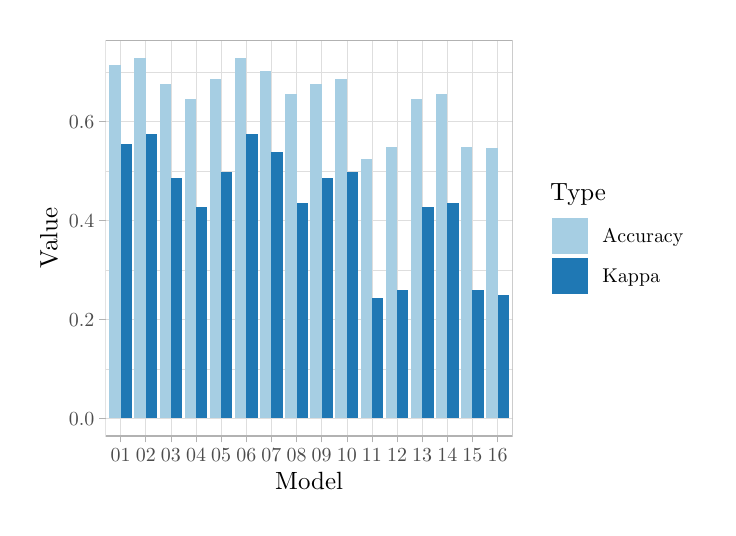
\begin{tikzpicture}[x=1pt,y=1pt]
\definecolor{fillColor}{RGB}{255,255,255}
\path[use as bounding box,fill=fillColor,fill opacity=0.00] (0,0) rectangle (245.72,173.45);
\begin{scope}
\path[clip] (  0.00,  0.00) rectangle (245.72,173.45);
\definecolor{drawColor}{RGB}{255,255,255}
\definecolor{fillColor}{RGB}{255,255,255}

\path[draw=drawColor,line width= 0.5pt,line join=round,line cap=round,fill=fillColor] (  0.00,  0.00) rectangle (245.72,173.45);
\end{scope}
\begin{scope}
\path[clip] ( 28.14, 25.85) rectangle (175.25,168.95);
\definecolor{fillColor}{RGB}{255,255,255}

\path[fill=fillColor] ( 28.14, 25.85) rectangle (175.25,168.95);
\definecolor{drawColor}{gray}{0.87}

\path[draw=drawColor,line width= 0.1pt,line join=round] ( 28.14, 50.22) --
	(175.25, 50.22);

\path[draw=drawColor,line width= 0.1pt,line join=round] ( 28.14, 85.96) --
	(175.25, 85.96);

\path[draw=drawColor,line width= 0.1pt,line join=round] ( 28.14,121.70) --
	(175.25,121.70);

\path[draw=drawColor,line width= 0.1pt,line join=round] ( 28.14,157.44) --
	(175.25,157.44);

\path[draw=drawColor,line width= 0.2pt,line join=round] ( 28.14, 32.35) --
	(175.25, 32.35);

\path[draw=drawColor,line width= 0.2pt,line join=round] ( 28.14, 68.09) --
	(175.25, 68.09);

\path[draw=drawColor,line width= 0.2pt,line join=round] ( 28.14,103.83) --
	(175.25,103.83);

\path[draw=drawColor,line width= 0.2pt,line join=round] ( 28.14,139.57) --
	(175.25,139.57);

\path[draw=drawColor,line width= 0.2pt,line join=round] ( 33.59, 25.85) --
	( 33.59,168.95);

\path[draw=drawColor,line width= 0.2pt,line join=round] ( 42.67, 25.85) --
	( 42.67,168.95);

\path[draw=drawColor,line width= 0.2pt,line join=round] ( 51.75, 25.85) --
	( 51.75,168.95);

\path[draw=drawColor,line width= 0.2pt,line join=round] ( 60.83, 25.85) --
	( 60.83,168.95);

\path[draw=drawColor,line width= 0.2pt,line join=round] ( 69.91, 25.85) --
	( 69.91,168.95);

\path[draw=drawColor,line width= 0.2pt,line join=round] ( 78.99, 25.85) --
	( 78.99,168.95);

\path[draw=drawColor,line width= 0.2pt,line join=round] ( 88.07, 25.85) --
	( 88.07,168.95);

\path[draw=drawColor,line width= 0.2pt,line join=round] ( 97.16, 25.85) --
	( 97.16,168.95);

\path[draw=drawColor,line width= 0.2pt,line join=round] (106.24, 25.85) --
	(106.24,168.95);

\path[draw=drawColor,line width= 0.2pt,line join=round] (115.32, 25.85) --
	(115.32,168.95);

\path[draw=drawColor,line width= 0.2pt,line join=round] (124.40, 25.85) --
	(124.40,168.95);

\path[draw=drawColor,line width= 0.2pt,line join=round] (133.48, 25.85) --
	(133.48,168.95);

\path[draw=drawColor,line width= 0.2pt,line join=round] (142.56, 25.85) --
	(142.56,168.95);

\path[draw=drawColor,line width= 0.2pt,line join=round] (151.64, 25.85) --
	(151.64,168.95);

\path[draw=drawColor,line width= 0.2pt,line join=round] (160.72, 25.85) --
	(160.72,168.95);

\path[draw=drawColor,line width= 0.2pt,line join=round] (169.80, 25.85) --
	(169.80,168.95);
\definecolor{fillColor}{RGB}{31,120,180}

\path[fill=fillColor] ( 33.59, 32.35) rectangle ( 37.68,131.28);
\definecolor{fillColor}{RGB}{166,206,227}

\path[fill=fillColor] ( 29.50, 32.35) rectangle ( 33.59,159.89);
\definecolor{fillColor}{RGB}{31,120,180}

\path[fill=fillColor] ( 42.67, 32.35) rectangle ( 46.76,134.95);
\definecolor{fillColor}{RGB}{166,206,227}

\path[fill=fillColor] ( 38.58, 32.35) rectangle ( 42.67,162.44);
\definecolor{fillColor}{RGB}{31,120,180}

\path[fill=fillColor] ( 51.75, 32.35) rectangle ( 55.84,119.06);
\definecolor{fillColor}{RGB}{166,206,227}

\path[fill=fillColor] ( 47.66, 32.35) rectangle ( 51.75,153.12);
\definecolor{fillColor}{RGB}{31,120,180}

\path[fill=fillColor] ( 60.83, 32.35) rectangle ( 64.92,108.72);
\definecolor{fillColor}{RGB}{166,206,227}

\path[fill=fillColor] ( 56.75, 32.35) rectangle ( 60.83,147.83);
\definecolor{fillColor}{RGB}{31,120,180}

\path[fill=fillColor] ( 69.91, 32.35) rectangle ( 74.00,121.41);
\definecolor{fillColor}{RGB}{166,206,227}

\path[fill=fillColor] ( 65.83, 32.35) rectangle ( 69.91,154.95);
\definecolor{fillColor}{RGB}{31,120,180}

\path[fill=fillColor] ( 78.99, 32.35) rectangle ( 83.08,134.95);
\definecolor{fillColor}{RGB}{166,206,227}

\path[fill=fillColor] ( 74.91, 32.35) rectangle ( 78.99,162.44);
\definecolor{fillColor}{RGB}{31,120,180}

\path[fill=fillColor] ( 88.07, 32.35) rectangle ( 92.16,128.39);
\definecolor{fillColor}{RGB}{166,206,227}

\path[fill=fillColor] ( 83.99, 32.35) rectangle ( 88.07,157.88);
\definecolor{fillColor}{RGB}{31,120,180}

\path[fill=fillColor] ( 97.16, 32.35) rectangle (101.24,110.25);
\definecolor{fillColor}{RGB}{166,206,227}

\path[fill=fillColor] ( 93.07, 32.35) rectangle ( 97.16,149.47);
\definecolor{fillColor}{RGB}{31,120,180}

\path[fill=fillColor] (106.24, 32.35) rectangle (110.32,119.06);
\definecolor{fillColor}{RGB}{166,206,227}

\path[fill=fillColor] (102.15, 32.35) rectangle (106.24,153.12);
\definecolor{fillColor}{RGB}{31,120,180}

\path[fill=fillColor] (115.32, 32.35) rectangle (119.40,121.41);
\definecolor{fillColor}{RGB}{166,206,227}

\path[fill=fillColor] (111.23, 32.35) rectangle (115.32,154.95);
\definecolor{fillColor}{RGB}{31,120,180}

\path[fill=fillColor] (124.40, 32.35) rectangle (128.48, 75.69);
\definecolor{fillColor}{RGB}{166,206,227}

\path[fill=fillColor] (120.31, 32.35) rectangle (124.40,126.08);
\definecolor{fillColor}{RGB}{31,120,180}

\path[fill=fillColor] (133.48, 32.35) rectangle (137.57, 78.74);
\definecolor{fillColor}{RGB}{166,206,227}

\path[fill=fillColor] (129.39, 32.35) rectangle (133.48,130.47);
\definecolor{fillColor}{RGB}{31,120,180}

\path[fill=fillColor] (142.56, 32.35) rectangle (146.65,108.72);
\definecolor{fillColor}{RGB}{166,206,227}

\path[fill=fillColor] (138.47, 32.35) rectangle (142.56,147.83);
\definecolor{fillColor}{RGB}{31,120,180}

\path[fill=fillColor] (151.64, 32.35) rectangle (155.73,110.25);
\definecolor{fillColor}{RGB}{166,206,227}

\path[fill=fillColor] (147.55, 32.35) rectangle (151.64,149.47);
\definecolor{fillColor}{RGB}{31,120,180}

\path[fill=fillColor] (160.72, 32.35) rectangle (164.81, 78.74);
\definecolor{fillColor}{RGB}{166,206,227}

\path[fill=fillColor] (156.64, 32.35) rectangle (160.72,130.47);
\definecolor{fillColor}{RGB}{31,120,180}

\path[fill=fillColor] (169.80, 32.35) rectangle (173.89, 77.02);
\definecolor{fillColor}{RGB}{166,206,227}

\path[fill=fillColor] (165.72, 32.35) rectangle (169.80,129.92);
\definecolor{drawColor}{gray}{0.70}

\path[draw=drawColor,line width= 0.5pt,line join=round,line cap=round] ( 28.14, 25.85) rectangle (175.25,168.95);
\end{scope}
\begin{scope}
\path[clip] (  0.00,  0.00) rectangle (245.72,173.45);
\definecolor{drawColor}{gray}{0.30}

\node[text=drawColor,anchor=base east,inner sep=0pt, outer sep=0pt, scale=  0.72] at ( 24.09, 29.87) {0.0};

\node[text=drawColor,anchor=base east,inner sep=0pt, outer sep=0pt, scale=  0.72] at ( 24.09, 65.61) {0.2};

\node[text=drawColor,anchor=base east,inner sep=0pt, outer sep=0pt, scale=  0.72] at ( 24.09,101.35) {0.4};

\node[text=drawColor,anchor=base east,inner sep=0pt, outer sep=0pt, scale=  0.72] at ( 24.09,137.09) {0.6};
\end{scope}
\begin{scope}
\path[clip] (  0.00,  0.00) rectangle (245.72,173.45);
\definecolor{drawColor}{gray}{0.70}

\path[draw=drawColor,line width= 0.2pt,line join=round] ( 25.89, 32.35) --
	( 28.14, 32.35);

\path[draw=drawColor,line width= 0.2pt,line join=round] ( 25.89, 68.09) --
	( 28.14, 68.09);

\path[draw=drawColor,line width= 0.2pt,line join=round] ( 25.89,103.83) --
	( 28.14,103.83);

\path[draw=drawColor,line width= 0.2pt,line join=round] ( 25.89,139.57) --
	( 28.14,139.57);
\end{scope}
\begin{scope}
\path[clip] (  0.00,  0.00) rectangle (245.72,173.45);
\definecolor{drawColor}{gray}{0.70}

\path[draw=drawColor,line width= 0.2pt,line join=round] ( 33.59, 23.60) --
	( 33.59, 25.85);

\path[draw=drawColor,line width= 0.2pt,line join=round] ( 42.67, 23.60) --
	( 42.67, 25.85);

\path[draw=drawColor,line width= 0.2pt,line join=round] ( 51.75, 23.60) --
	( 51.75, 25.85);

\path[draw=drawColor,line width= 0.2pt,line join=round] ( 60.83, 23.60) --
	( 60.83, 25.85);

\path[draw=drawColor,line width= 0.2pt,line join=round] ( 69.91, 23.60) --
	( 69.91, 25.85);

\path[draw=drawColor,line width= 0.2pt,line join=round] ( 78.99, 23.60) --
	( 78.99, 25.85);

\path[draw=drawColor,line width= 0.2pt,line join=round] ( 88.07, 23.60) --
	( 88.07, 25.85);

\path[draw=drawColor,line width= 0.2pt,line join=round] ( 97.16, 23.60) --
	( 97.16, 25.85);

\path[draw=drawColor,line width= 0.2pt,line join=round] (106.24, 23.60) --
	(106.24, 25.85);

\path[draw=drawColor,line width= 0.2pt,line join=round] (115.32, 23.60) --
	(115.32, 25.85);

\path[draw=drawColor,line width= 0.2pt,line join=round] (124.40, 23.60) --
	(124.40, 25.85);

\path[draw=drawColor,line width= 0.2pt,line join=round] (133.48, 23.60) --
	(133.48, 25.85);

\path[draw=drawColor,line width= 0.2pt,line join=round] (142.56, 23.60) --
	(142.56, 25.85);

\path[draw=drawColor,line width= 0.2pt,line join=round] (151.64, 23.60) --
	(151.64, 25.85);

\path[draw=drawColor,line width= 0.2pt,line join=round] (160.72, 23.60) --
	(160.72, 25.85);

\path[draw=drawColor,line width= 0.2pt,line join=round] (169.80, 23.60) --
	(169.80, 25.85);
\end{scope}
\begin{scope}
\path[clip] (  0.00,  0.00) rectangle (245.72,173.45);
\definecolor{drawColor}{gray}{0.30}

\node[text=drawColor,anchor=base,inner sep=0pt, outer sep=0pt, scale=  0.72] at ( 33.59, 16.84) {01};

\node[text=drawColor,anchor=base,inner sep=0pt, outer sep=0pt, scale=  0.72] at ( 42.67, 16.84) {02};

\node[text=drawColor,anchor=base,inner sep=0pt, outer sep=0pt, scale=  0.72] at ( 51.75, 16.84) {03};

\node[text=drawColor,anchor=base,inner sep=0pt, outer sep=0pt, scale=  0.72] at ( 60.83, 16.84) {04};

\node[text=drawColor,anchor=base,inner sep=0pt, outer sep=0pt, scale=  0.72] at ( 69.91, 16.84) {05};

\node[text=drawColor,anchor=base,inner sep=0pt, outer sep=0pt, scale=  0.72] at ( 78.99, 16.84) {06};

\node[text=drawColor,anchor=base,inner sep=0pt, outer sep=0pt, scale=  0.72] at ( 88.07, 16.84) {07};

\node[text=drawColor,anchor=base,inner sep=0pt, outer sep=0pt, scale=  0.72] at ( 97.16, 16.84) {08};

\node[text=drawColor,anchor=base,inner sep=0pt, outer sep=0pt, scale=  0.72] at (106.24, 16.84) {09};

\node[text=drawColor,anchor=base,inner sep=0pt, outer sep=0pt, scale=  0.72] at (115.32, 16.84) {10};

\node[text=drawColor,anchor=base,inner sep=0pt, outer sep=0pt, scale=  0.72] at (124.40, 16.84) {11};

\node[text=drawColor,anchor=base,inner sep=0pt, outer sep=0pt, scale=  0.72] at (133.48, 16.84) {12};

\node[text=drawColor,anchor=base,inner sep=0pt, outer sep=0pt, scale=  0.72] at (142.56, 16.84) {13};

\node[text=drawColor,anchor=base,inner sep=0pt, outer sep=0pt, scale=  0.72] at (151.64, 16.84) {14};

\node[text=drawColor,anchor=base,inner sep=0pt, outer sep=0pt, scale=  0.72] at (160.72, 16.84) {15};

\node[text=drawColor,anchor=base,inner sep=0pt, outer sep=0pt, scale=  0.72] at (169.80, 16.84) {16};
\end{scope}
\begin{scope}
\path[clip] (  0.00,  0.00) rectangle (245.72,173.45);
\definecolor{drawColor}{RGB}{0,0,0}

\node[text=drawColor,anchor=base,inner sep=0pt, outer sep=0pt, scale=  0.90] at (101.70,  6.44) {Model};
\end{scope}
\begin{scope}
\path[clip] (  0.00,  0.00) rectangle (245.72,173.45);
\definecolor{drawColor}{RGB}{0,0,0}

\node[text=drawColor,rotate= 90.00,anchor=base,inner sep=0pt, outer sep=0pt, scale=  0.90] at ( 10.70, 97.40) {Value};
\end{scope}
\begin{scope}
\path[clip] (  0.00,  0.00) rectangle (245.72,173.45);
\definecolor{fillColor}{RGB}{255,255,255}

\path[fill=fillColor] (184.25, 72.12) rectangle (241.22,122.67);
\end{scope}
\begin{scope}
\path[clip] (  0.00,  0.00) rectangle (245.72,173.45);
\definecolor{drawColor}{RGB}{0,0,0}

\node[text=drawColor,anchor=base west,inner sep=0pt, outer sep=0pt, scale=  0.90] at (188.75,111.00) {Type};
\end{scope}
\begin{scope}
\path[clip] (  0.00,  0.00) rectangle (245.72,173.45);
\definecolor{fillColor}{RGB}{255,255,255}

\path[fill=fillColor] (188.75, 91.08) rectangle (203.21,105.53);
\end{scope}
\begin{scope}
\path[clip] (  0.00,  0.00) rectangle (245.72,173.45);
\definecolor{fillColor}{RGB}{166,206,227}

\path[fill=fillColor] (189.46, 91.79) rectangle (202.49,104.82);
\end{scope}
\begin{scope}
\path[clip] (  0.00,  0.00) rectangle (245.72,173.45);
\definecolor{fillColor}{RGB}{255,255,255}

\path[fill=fillColor] (188.75, 76.62) rectangle (203.21, 91.08);
\end{scope}
\begin{scope}
\path[clip] (  0.00,  0.00) rectangle (245.72,173.45);
\definecolor{fillColor}{RGB}{31,120,180}

\path[fill=fillColor] (189.46, 77.33) rectangle (202.49, 90.36);
\end{scope}
\begin{scope}
\path[clip] (  0.00,  0.00) rectangle (245.72,173.45);
\definecolor{drawColor}{RGB}{0,0,0}

\node[text=drawColor,anchor=base west,inner sep=0pt, outer sep=0pt, scale=  0.72] at (207.71, 95.82) {Accuracy};
\end{scope}
\begin{scope}
\path[clip] (  0.00,  0.00) rectangle (245.72,173.45);
\definecolor{drawColor}{RGB}{0,0,0}

\node[text=drawColor,anchor=base west,inner sep=0pt, outer sep=0pt, scale=  0.72] at (207.71, 81.37) {Kappa};
\end{scope}
\end{tikzpicture}
